\setlength{\footskip}{8mm}

\chapter{Results}

\label{ch:results}

This chapter describes the results obtained with this research.
First, the deep neural network model used in the study is described. Then, the results obtained with this network in the context of face verification are given. Finally, we will describe the final experimental software which is available online and the results one can expect with it.

\section{Preliminary results}
Before the proposal, some parts of the solution have been built.
\begin{itemize}
\item Scripts to generate the database of face images from a video surveillance sequence have been written. The database has been generated and is usable for a direct face identification model. However, the overlap calculation for face detection is not written yet. Hence, the number of available classes is limited, decreasing the performances of a \enquote{Same/Not Same} network. The direct face identification model is not be affected by this issue, however it can be built with the current version of the database. The database contains 55,203 images. After manual labeling of the faces in the database, 183 images were labeled 1 for the first researcher, 325 were labeled 2, 15 were labeled 3.
\item The scripts to generate the database files mentioned in Figure 3.2 are fully written, and work both for a direct face identification and for a Siamese network. They were executed for this second scenario. Four files \enquote{train1.txt}, \enquote{train2.txt}, \enquote{test1.txt}, and \enquote{test2.txt}, as described in section 3.6.2, were built.
\item A Siamese model has been designed with Caffe and was trained on the generated database for 50,000 epochs. This training took a night, with batches of size 20, on the 780 GTX GPU card given by the laboratory. The accuracy of the resulting network could not be tested yet because of the singular output generated by such a network, as mentioned in section 2.3.1. A script is being written to face this issue.
\end{itemize}

\section{Network used in this research}

Wu, He and Sun published a light convolutional neural network for face verification (November 2015). Its particularity is that it is extremely light but still reaches state-of-the-art results.

\subsection{Architecture}
The following figure describes its architecture.

\begin{figure}[!ht]
  \centering
  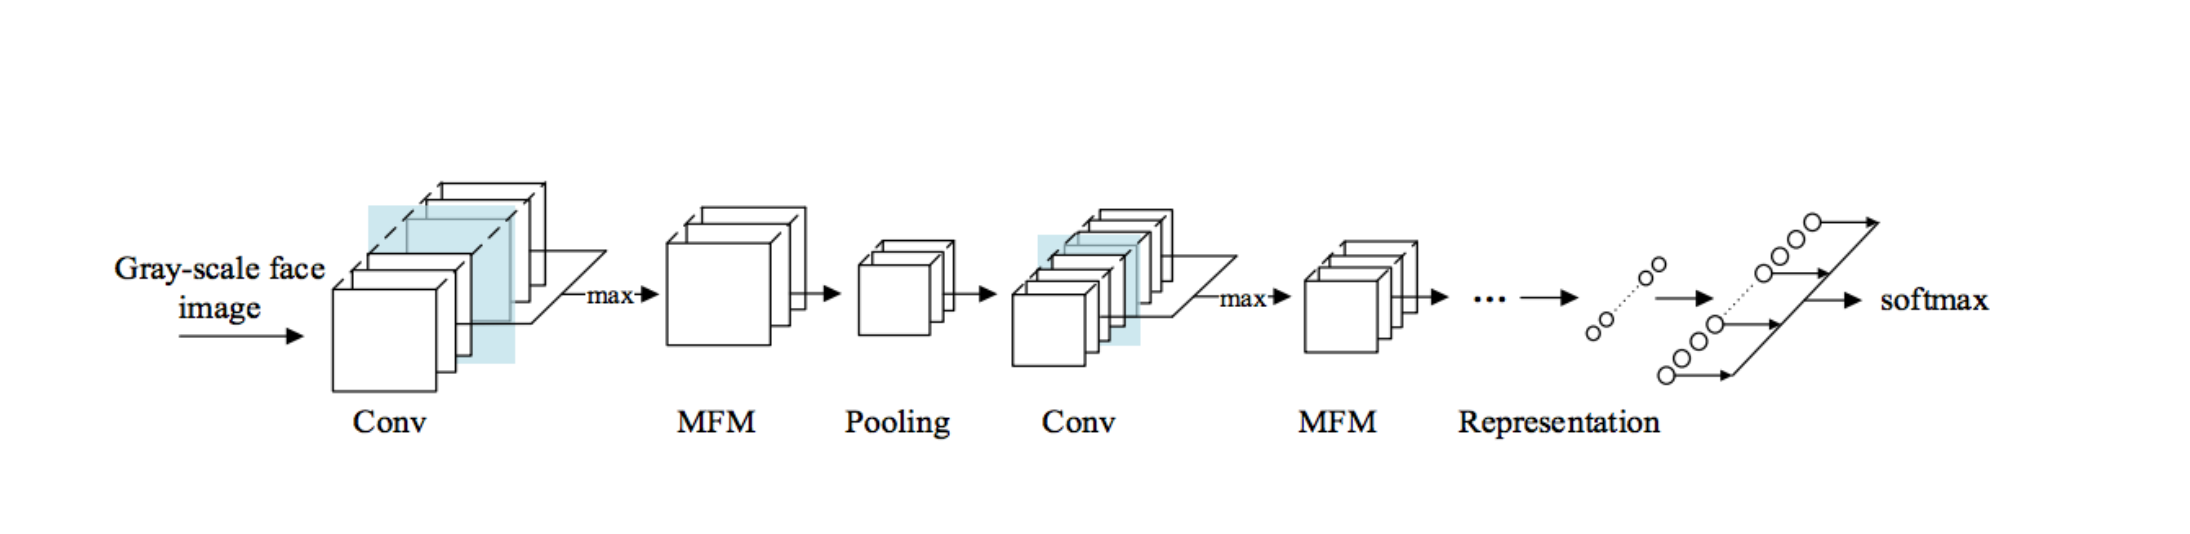
\includegraphics[scale=0.4]{figures/final_net.png}  
  \caption[Architecture of the lightened convolution network. Extracted from Wu, He, Sun, 2015.]{Architecture of the lightened convolution network. Extracted from Wu, He, Sun, 2015.}
  \protect\label{fig:Siamese}
\end{figure}
\FloatBarrier
\end{itemize}

First, as an input, a Gray-scale face image is provided. The article suggests the use of two possible models. The one used in this research is built with 4 convolution layer with Max-Feature-Map activation functions, 4 max-pooling layers and 2 fully connected layers. The details are given in the following figure.

\begin{figure}[!ht]
  \centering
  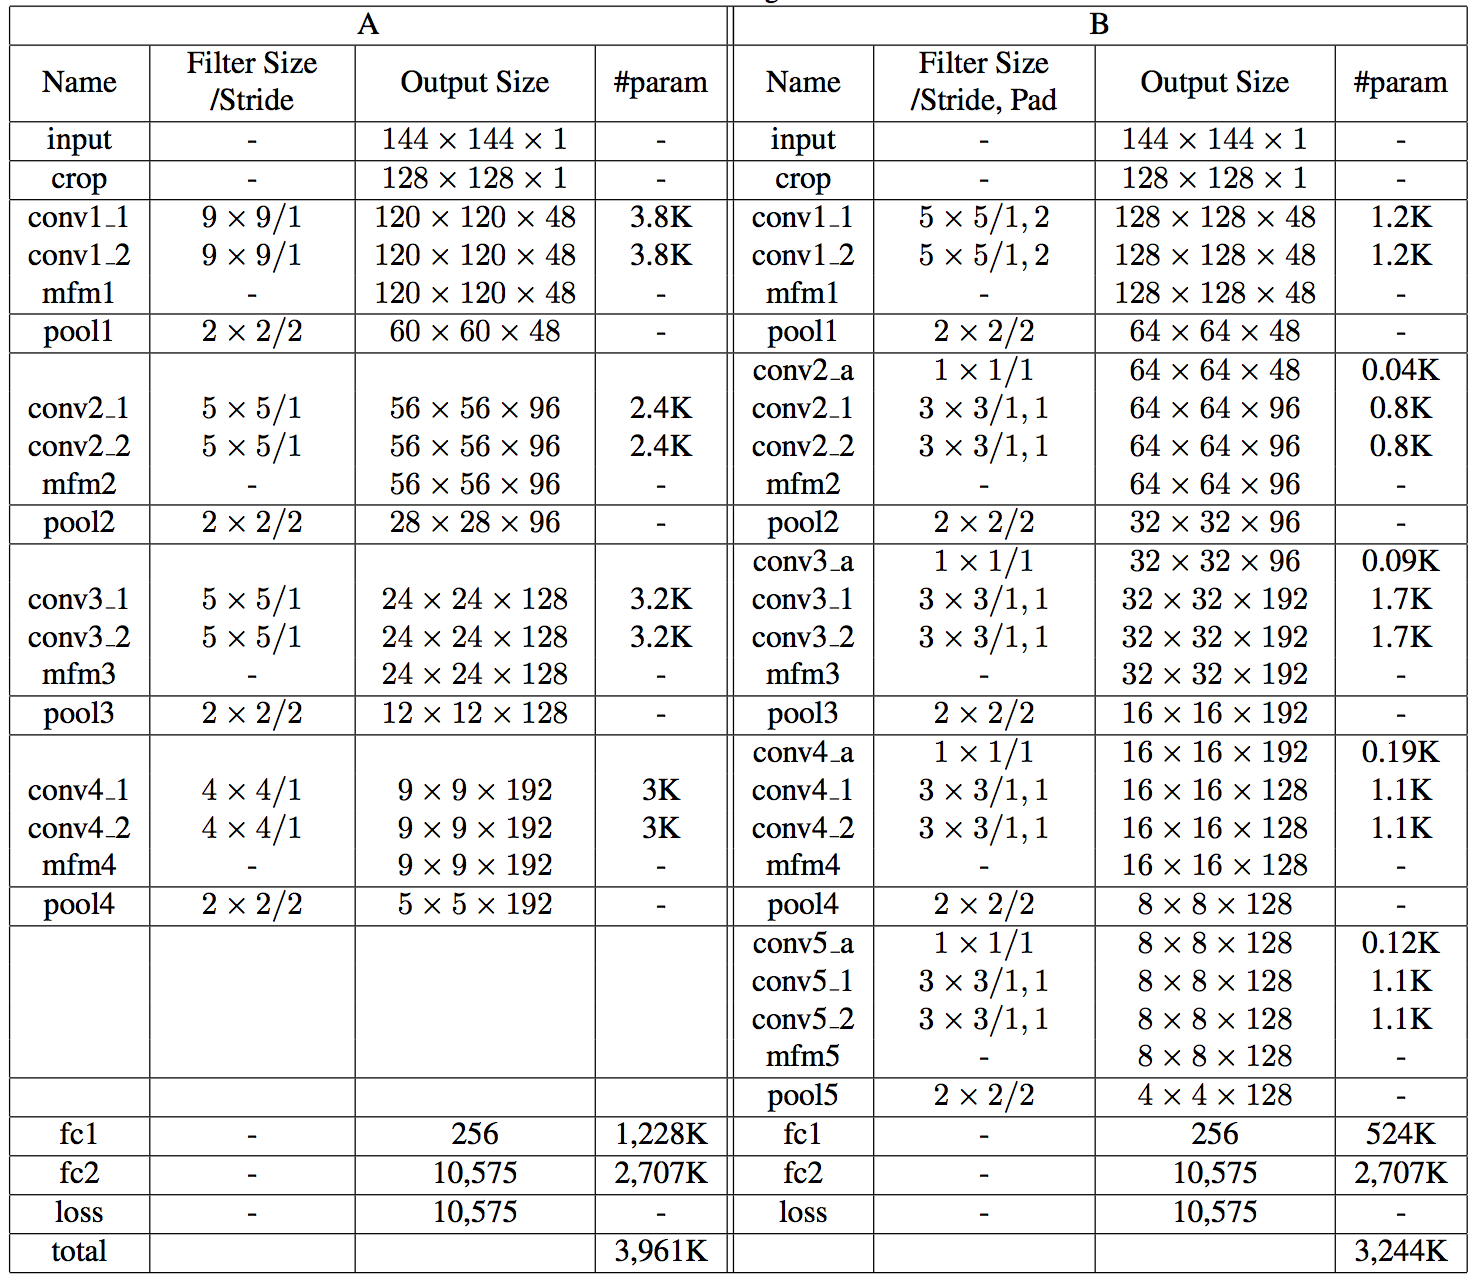
\includegraphics[scale=0.6]{figures/architecture.png}  
  \protect\label{fig:architecture}
  \caption[Details on the architecture of the lightened convolution networks. Extracted from Wu, He, Sun, 2015.]{Details on the architecture of the lightened convolution networks. Extracted from Wu, He, Sun, 2015.}
\end{figure}
\FloatBarrier
\end{itemize}

\FloatBarrier

The MFM function works as explained in the following figure.

\begin{figure}[!ht]
  \centering
  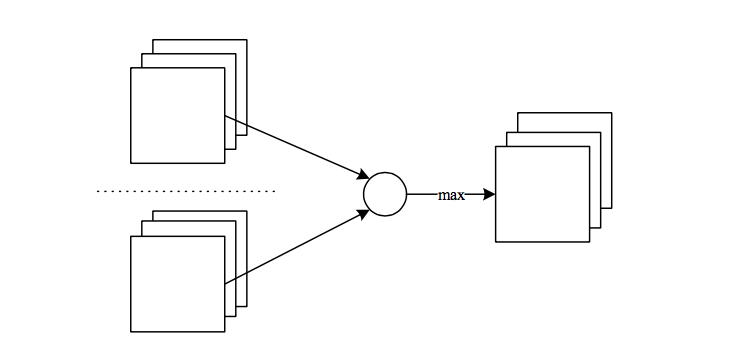
\includegraphics[scale=0.4]{figures/mfm.png}  
  \protect\label{fig:mfm}
  \caption[The MFM activation function used on a convolution layer. Extracted from Wu, He, Sun, 2015.]{The MFM activation function on a convolution layer. Extracted from Wu, He, Sun, 2015.}
\end{figure}
\FloatBarrier
\end{itemize}

\FloatBarrier

Given a convolution layer \(C \in R^h^w^2^n\), the MFM can be written :

\begin{figure}[!ht]
  \centering
  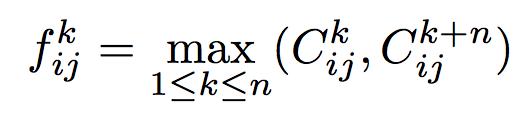
\includegraphics[scale=0.4]{figures/equ.png}  
  \protect\label{fig:equ}
\end{figure}
\FloatBarrier
\end{itemize}

\FloatBarrier

\(2n\) being the channel of the input convolution layer, \(1 \leq i \leq h\) and \(1 \leq j \leq w\).

Given a face image as an input, the output of the neural network is an array of float values called features. To verify that the face on an image is the same as the face on another one, the cosine of their corresponding feature array is computed and is compared to a threshold.

\subsection{Results}

As said previously, these networks reach state-of-the-art results. The two networks were trained on the LFW database and tested both on LFW and YTF (YouTube Faces Database). The results are given in the next two tables, compared with other state-of-the-art methods.

\begin{figure}[!ht]
  \centering
  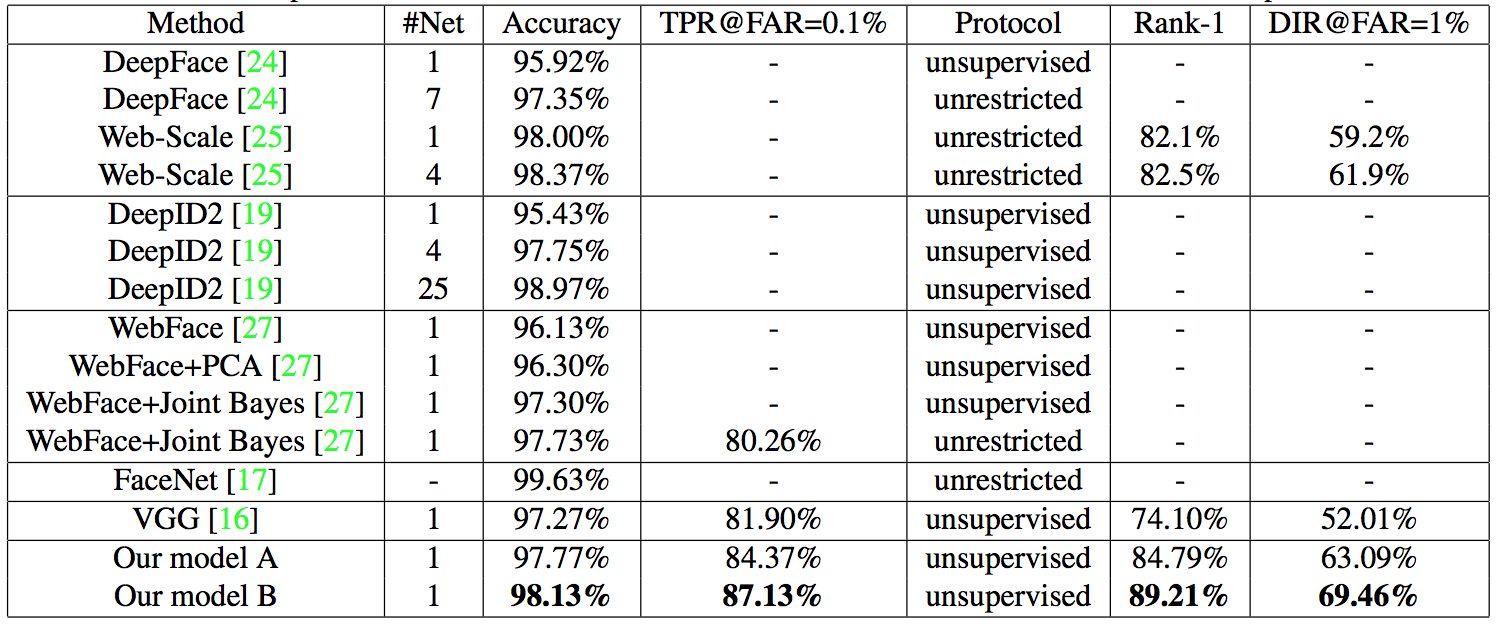
\includegraphics[scale=0.6]{figures/lfw.png}  
  \protect\label{fig:mfm}
  \caption[Comparison with other state-of-the-art methods on LFW. Extracted from Wu, He, Sun, 2015.]{Comparison with other state-of-the-art methods on LFW. Extracted from Wu, He, Sun, 2015.}
\end{figure}
\FloatBarrier
\end{itemize}


\begin{figure}[!ht]
  \centering
  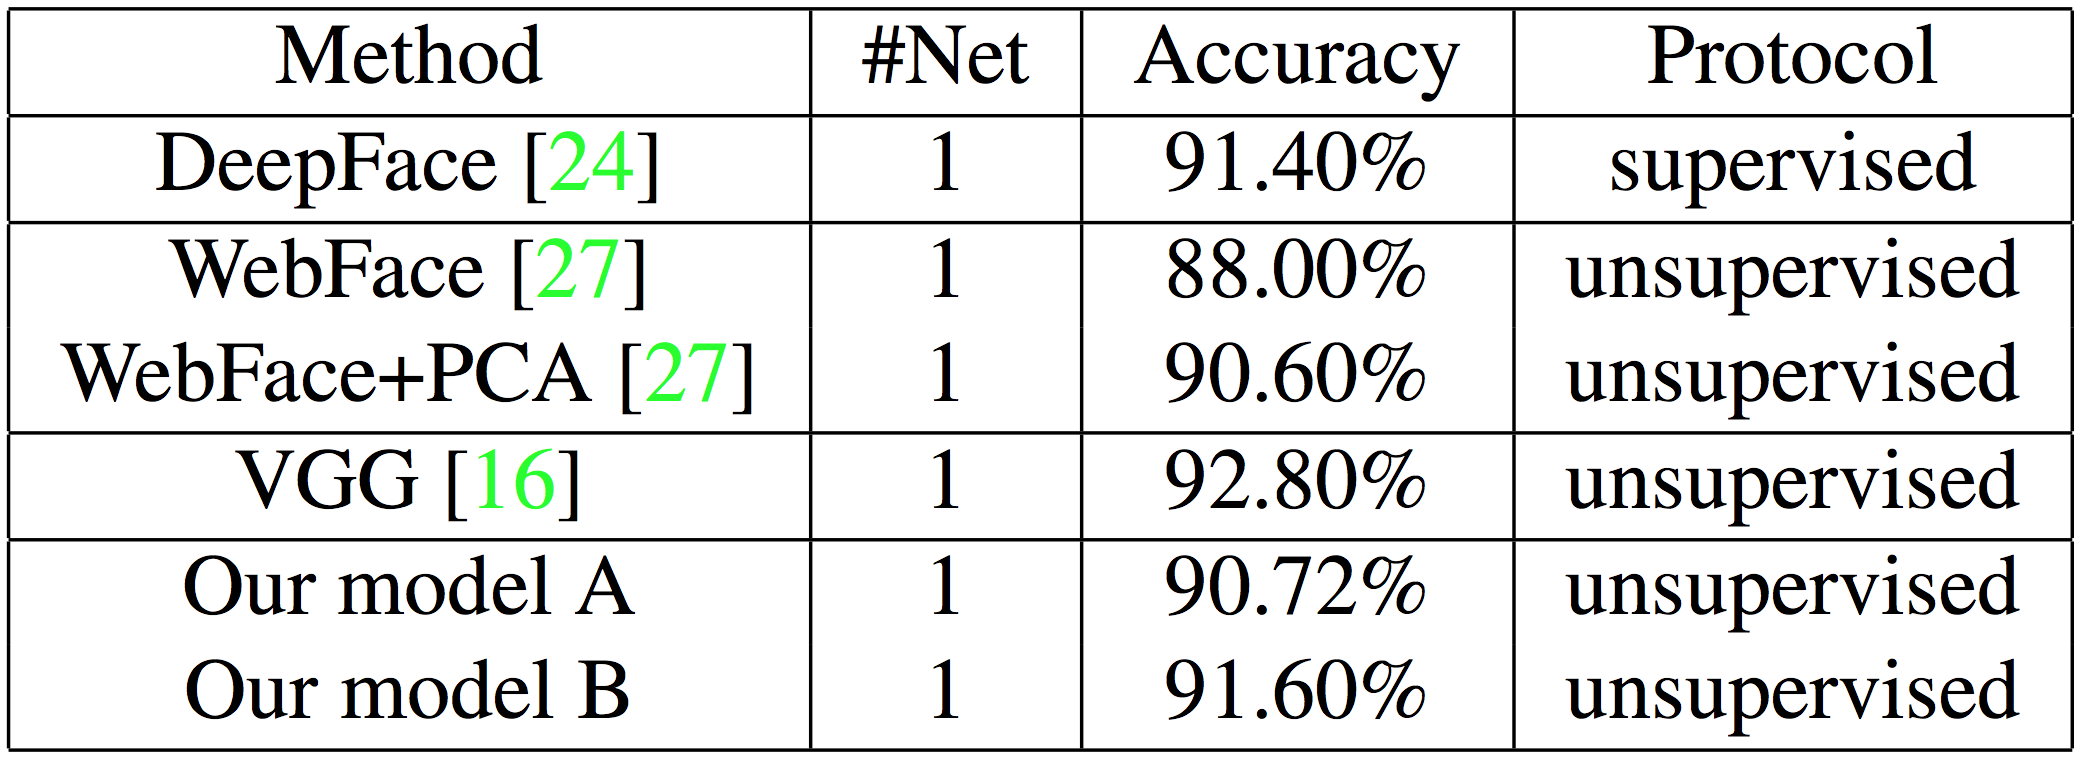
\includegraphics[scale=0.3]{figures/ytf.png}  
  \protect\label{fig:mfm}
  \caption[Comparison with other state-of-the-art methods on YTF. Extracted from Wu, He, Sun, 2015.]{Comparison with other state-of-the-art methods on YTF. Extracted from Wu, He, Sun, 2015.}
\end{figure}
\FloatBarrier
\end{itemize}

\FloatBarrier

\section{Results on the MBK database}
\subsection{The MBK database}
The MBK database is an experimental database of faces extracted from surveillance videos in the MBK mall in Bangkok. The labeling of the faces is done both through automatic overlapping and manual labeling for the researchers. This leads to around 85,000 images of faces. Few mistakes were made by the automatic process and it was not feasible to correct them. Furthermore, the faces are directly extracted from frames and their resolution is often very poor while their blurriness is important. 
\subsection{Test}
The network A presented in the previous section and pre-trained for the LFW database was used on this database of face images from surveillance video. It was tested on 13881 negative pairs and 13881 positive pairs. The first element of each pair was taken in the direct order of the database. The second element was taken such that each first element was the origin of as many positive and negative pairs. The negative pairs were chosen randomly.
\subsection{Result}
The ROC curve obtained is shown in the following figure. The accuracy of the model reaches 88.04\%.

\begin{figure}[!ht]
  \centering
  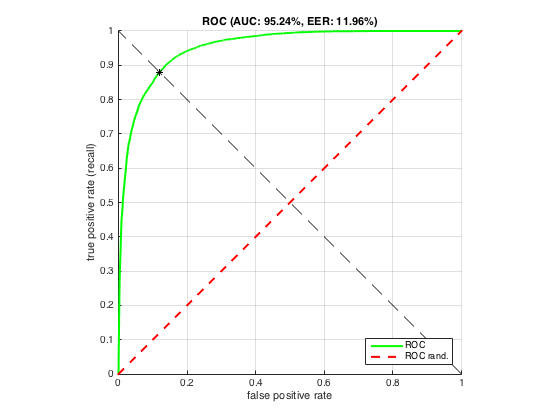
\includegraphics[scale=0.7]{figures/result.png}  
  \protect\label{fig:mfm}
  \caption[ROC curve of the network on the MBK database.]{ROC curve of the network on the MBK database.}
\end{figure}
\FloatBarrier
\end{itemize}

The ROC curve obtained on the MBK database is compared with other newtorks such as DeepFace on YTF database in the following figure. This comparison is a simple indication as the curves do not concern the same databases, though they are both made of face images extracted from videos. The light green one is the one from the MBK database, the others are all from YTF.

\begin{figure}[!ht]
  \centering
  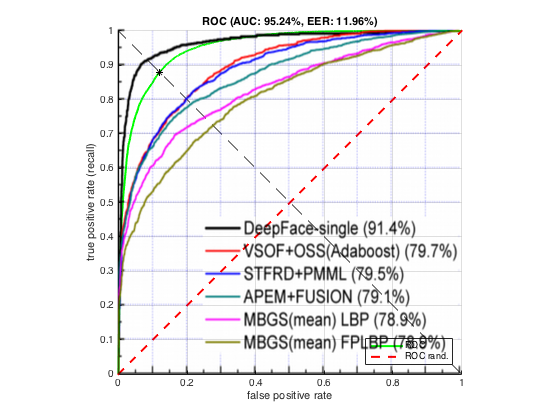
\includegraphics[scale=0.7]{figures/result_compared.png}  
  \protect\label{fig:mfm}
  \caption[ROC curve of the network on the MBK database.]{ROC curve of the network on the MBK database.}
\end{figure}
\FloatBarrier
\end{itemize}

A histogram describing the repartition of the positive and negative pairs relatively to their score is also provided. In blue are represented the negative pairs and in red are represented the positive ones. Few errors on the automatic process of overlapping were made. The details and the consequences of these errors are described in the next section.

\begin{figure}[!ht]
  \centering
  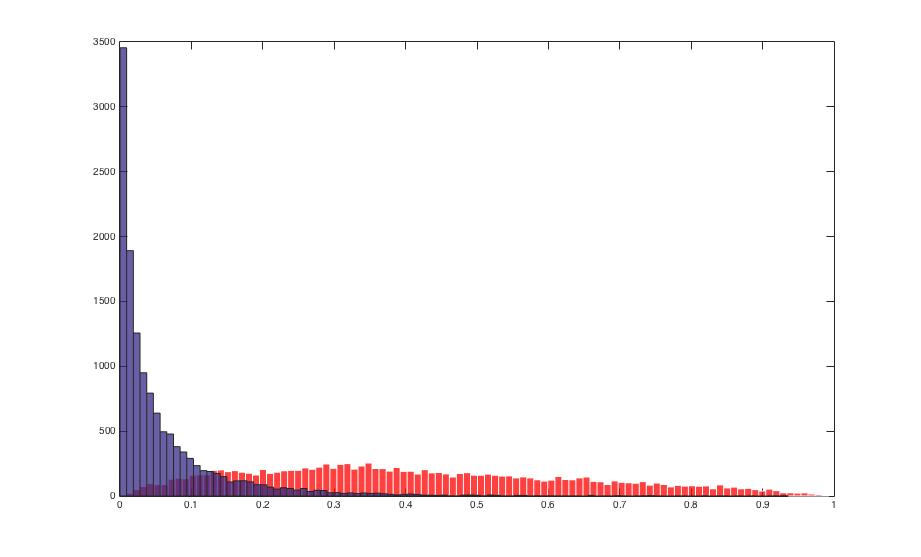
\includegraphics[scale=0.7]{figures/histograms.png}  
  \protect\label{fig:mfm}
  \caption[ROC curve of the network on the MBK database.]{ROC curve of the network on the MBK database.}
\end{figure}
\FloatBarrier
\end{itemize}
\FloatBarrier

\section{Description of the final product}

The final experimental product proposed at the end of this study is made of several parts.

\subsection{Face detection & overlapping}
As said in the third chapter, the face detection algorithm was written with C++ and OpenCV. The algorithm uses Haar feature-based cascade classifiers, described by Viola and Jones (2001). However a simple face detector was not enough and an overlapping algorithm providing automatic labeling of the faces had to be written for two reasons.
\begin{itemize}
\item First, to test the network we needed positive and negative pairs of images. The problem being that there are almost 90,000 images of faces in the database after the face detection was done and it was not possible to create enough pairs manually.
\item The second point is described in the last section of this chapter.
\end{itemize}
Consequently, an algorithm was written. Its behavior is described in pseudo-code:

\begin{algorithm}[H]
\For{each video in the database}{
 \For{each frame of the current video}{
  Detect all the faces of the frame N\;
 \For{each face of the current frame}{
    \If{there is a face detected in the three previous frames whose distance with the current face is inferior to the size of the face}{
    The label L of the current face := The label of the nearest of the faces of the three previous frames\;
    Save the detected face in \enquote{Database/video/LabelLFrameNFaceP.jpg}\;
    }
    \Else{}{
    The label L of the current face := Biggest label given until now + 1
    Save the detected face in \enquote{Database/video/LabelLFrameNFaceP.jpg}\;
    }
  }
  }
  }
 \caption{Automatic Labeling Algorithm}
\end{algorithm}

A representation of the final database is given below:


\begin{figure}[!ht]
  \centering
  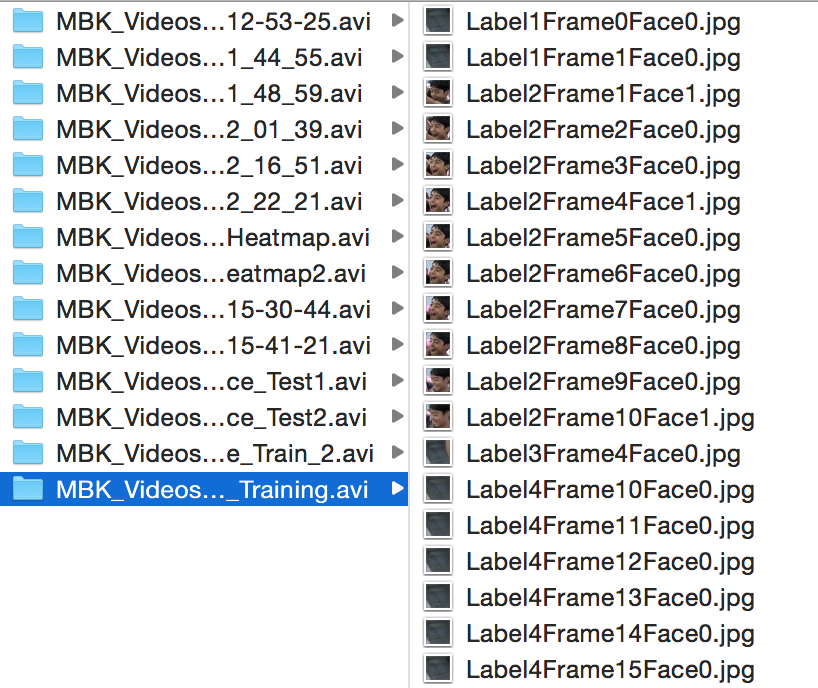
\includegraphics[scale=0.7]{figures/databaserepresentation.png}  
  \caption[The database after automatic labeling.]{The database after automatic labeling.}
  \protect\label{fig:Siamese}
\end{figure}
\FloatBarrier
\end{itemize}

This algorithm is efficient enough in our case but no study has been made on its real accuracy. Practically, two errors can be made.
\begin{itemize}
\item A single face appearing on the video is considered with two different labels.
\item Several faces appearing on the video are considered with the same label.
\end{itemize}

The first error does not change much about the results of the study. The negative pairs are chosen randomly in the list of all the faces. The possibility that two images from the same person are considered as negative pairs is very low. However the second scenario, more rare but still existing, is more dangerous for the precision of the analysis of the results as the positive pairs are created with all the available images of the same label. Consequently, the number of pairs considered as positive with a relatively low score is slightly overestimated while the number of pairs with a relatively low score is slightly underestimated. The global accuracy of the product is slightly underestimated.

\subsection{Face verification}
After the face detection process is done, the second part of the product can start.
It performs several successive actions.
\begin{itemize}
\item Asks the user to enter the address of the images of the person he is looking for in the database.
\item Process those images in the neural network which outputs an array of features (numbers) from each image. The above-mentioned distance between two images is directly computed as a cosine-score of their two corresponding arrays of features.
\item Asks for the address of the database containing the images of face.
\item The array of features of each image is computed by feed-forwarding the image in the neural network. The cosine-score of each image of detected face with each image of the person the user is looking for is computed. The algorithm decides whether it represents the same person or not.
\end{itemize}
\subsection{Selection of the best test}
For the rest of this chapter, let's call the detected images The initial naive idea was to consider that if each image